\documentclass[tikz,crop]{standalone}
\usepackage{amsmath}
\usepackage{amssymb}
\usepackage[english]{babel}
\usepackage[utf8]{inputenc}
\usepackage[T1]{fontenc}
\usepackage{euler}

\usepackage{tikz,pgfplots}
\usetikzlibrary{matrix, shapes, arrows, positioning}

\begin{document}

	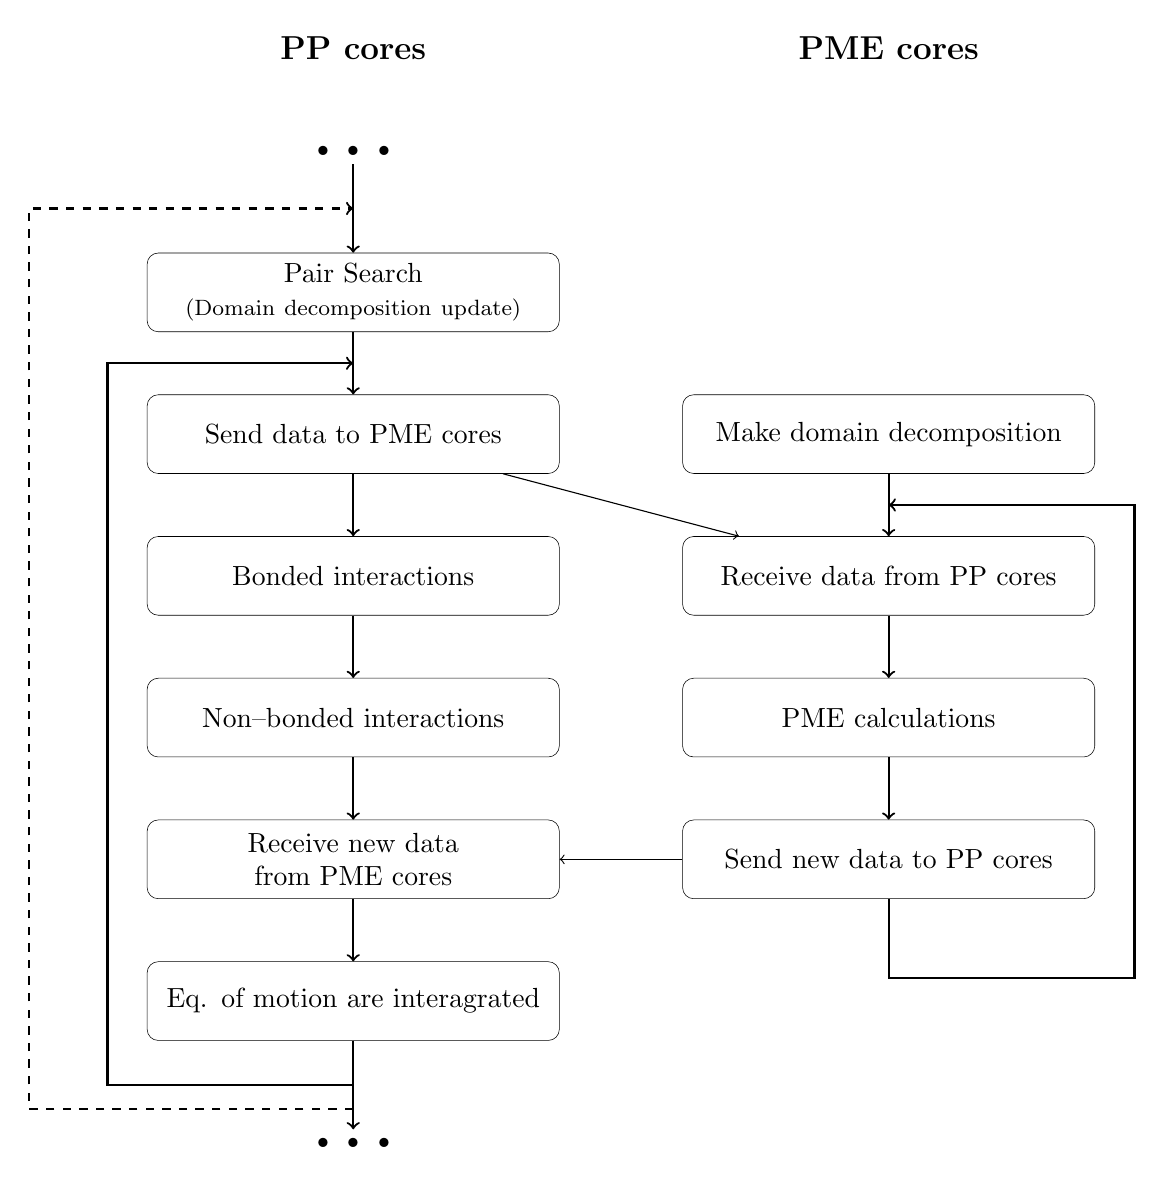
\begin{tikzpicture}[node distance=1.8cm]
		\node[align=center] (start) {\large\textbf{PP cores}};
		\node[align=center, right of=start, xshift=5cm] {\large\textbf{PME cores}};
		
		\node[align=center, below of=start, yshift=0.5cm] (0) {\Huge$\ldots$};
		\node[rectangle,draw,rounded corners,very thin,minimum width=5cm,minimum height=1cm,text width=5cm,align=center, below of=0] (A) {Pair Search \\ \footnotesize{(Domain decomposition update)}};
		
		%\node[rectangle,draw,rounded corners,very thin,minimum width=5cm,minimum height=1cm,text width=5cm,align=center, right of=A, xshift=5cm] (A1) {Make domain decomposition};
		
		\node[rectangle,draw,rounded corners,very thin,minimum width=5cm,minimum height=1cm,text width=5cm,align=center, below of=A] (B) {Send data to PME cores};
		
		\node[rectangle,draw,rounded corners,very thin,minimum width=5cm,minimum height=1cm,text width=5cm,align=center, right of=B, xshift=5cm] (B1) {Make domain decomposition};
		
		\node[rectangle,draw,rounded corners,very thin,minimum width=5cm,minimum height=1cm,text width=5cm,align=center, below of=B] (C) {Bonded interactions};
		
		\node[rectangle,draw,rounded corners,very thin,minimum width=5cm,minimum height=1cm,text width=5cm,align=center, right of=C, xshift=5cm] (C1) {Receive data from PP cores};
		
		\node[rectangle,draw,rounded corners,very thin,minimum width=5cm,minimum height=1cm,text width=5cm,align=center, below of=C] (D) {Non--bonded interactions};
		
		\node[rectangle,draw,rounded corners,very thin,minimum width=5cm,minimum height=1cm,text width=5cm,align=center, right of=D, xshift=5cm] (D1) {PME calculations};
		
		\node[rectangle,draw,rounded corners,very thin,minimum width=5cm,minimum height=1cm,text width=5cm,align=center, below of=D] (E) {Receive new data from PME cores};
		
		\node[rectangle,draw,rounded corners,very thin,minimum width=5cm,minimum height=1cm,text width=5cm,align=center, right of=E, xshift=5cm] (E1) {Send new data to PP cores};
		
		\node[rectangle,draw,rounded corners,very thin,minimum width=5cm,minimum height=1cm,text width=5cm,align=center, below of=E] (F) {Eq. of motion are interagrated};
		
		\node[align=center, below of=F] (G) {\Huge$\ldots$};
		
		\draw[thick,->] (0) -- (A) node[midway] (0A) {};
		\draw[thick,->] (A) -- (B) node[midway] (AB) {};
		\draw[thick,->] (B) -- (C);
		\draw[thick,->] (C) -- (D);
		\draw[thick,->] (D) -- (E);
		\draw[thick,->] (E) -- (F);
		\draw[thick,->] (F) -- (G) node[midway] (FG) {};
		
		\draw[thick,->] (FG.center) -| ([xshift=-0.5cm]B.west) |- (AB.center);
		\draw[thick,dashed,->] ([yshift=-0.3cm]FG.center) -| ([xshift=-1.5cm]A.west) |- (0A.center);
		
		%\draw[thick,->] (A1) -- (B1);
		\draw[thick,->] (B1) -- (C1) node[midway] (B1C1) {};
		\draw[thick,->] (C1) -- (D1);
		\draw[thick,->] (D1) -- (E1);
		
		\draw[->] (B) -- (C1);
		\draw[->] (E1) -- (E);
		
		\draw[thick,->] (E1.south) -- ([yshift=-1cm] E1.south) -| ([xshift=0.5cm]C1.east) |- (B1C1.center);

	\end{tikzpicture}
		
\end{document}
	